\documentclass[titlepage, 12pt]{article}

\usepackage{enumitem}
\usepackage{geometry}
\geometry{
  letterpaper,
  margin=1in,
}
\usepackage{graphicx}
\graphicspath{{./images/}}

\title{SE 2XB3 Group 4 Report 1}
\author{
  Huang, Kehao \\
  400235182 \\
  \texttt{huangk53@mcmaster.ca} \\
  L01
  \and
  Jiao, Anhao \\
  400251837 \\
  \texttt{jaoa3@mcmaster.ca} \\
  L01
  \and
  Ye, Xunzhou \\
  400268576 \\
  \texttt{yex33@mcmaster.ca} \\
  L01
}
\date{22 January 2021}

\begin{document}

\maketitle{}

\section*{Team Contract}
\label{sec:contract}

\begin{itemize}
\item We will primarily be using Discord to communicate.
\item All members must respond to messages which they are mentioned in within 2
  hours.
\item During 3:30pm--5:30pm on Mondays, all members must present in a Discord
  meeting to prepare for the lab on Tuesday.
\item During the assigned lab period on Tuesdays 8:30am--11:20am, all members
  must present in a Discord meeting to work on the lab.
\end{itemize}

\newpage{}

\section{Version Control}
\label{sec:git}

\subsection{Experiment 1: Push and Pull}
All group members successfully pushed their new files to the remote repository
and pulled the files created by other group members from the remote repository.
\begin{figure}[h]
  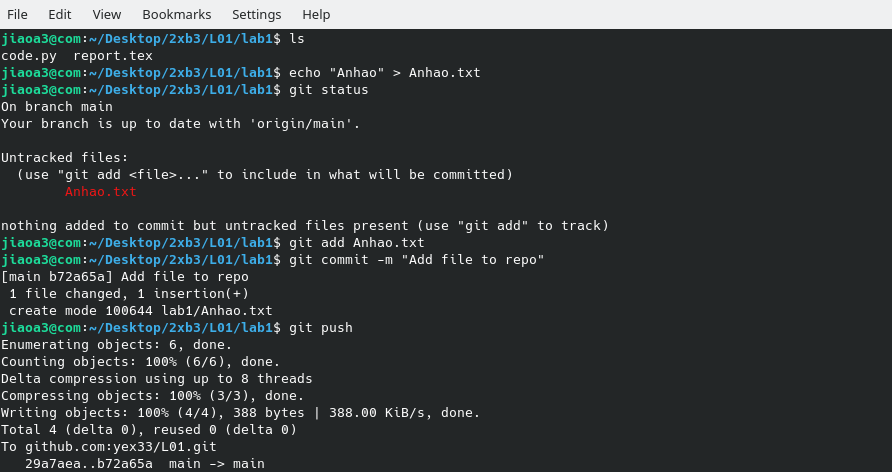
\includegraphics[width=\textwidth]{e1m1}
  \caption{Member 1}
\end{figure}
\begin{figure}[h]
  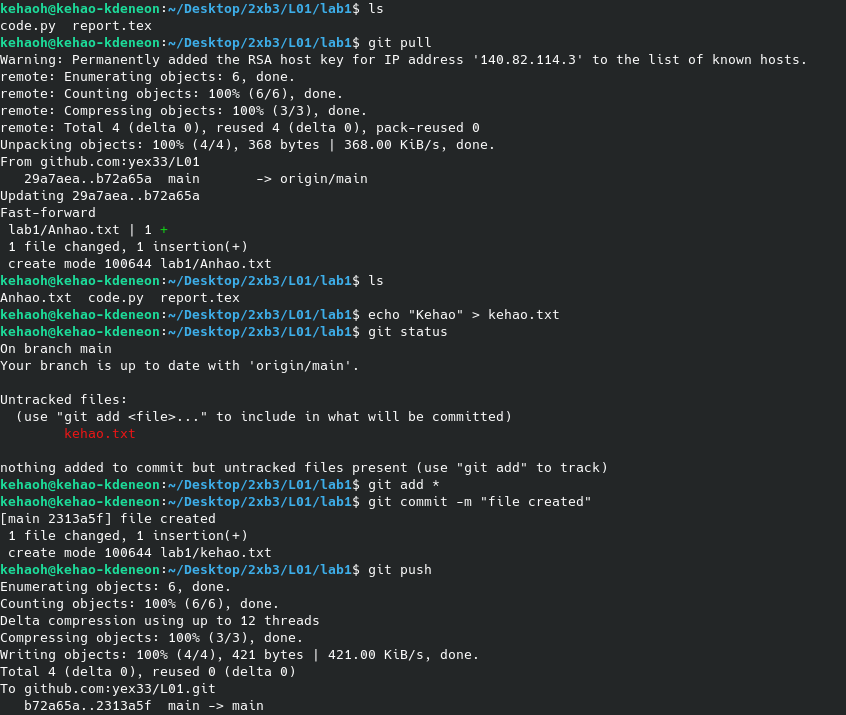
\includegraphics[width=\textwidth]{e1m2}
  \caption{Member 2}
\end{figure}
\begin{figure}[h]
  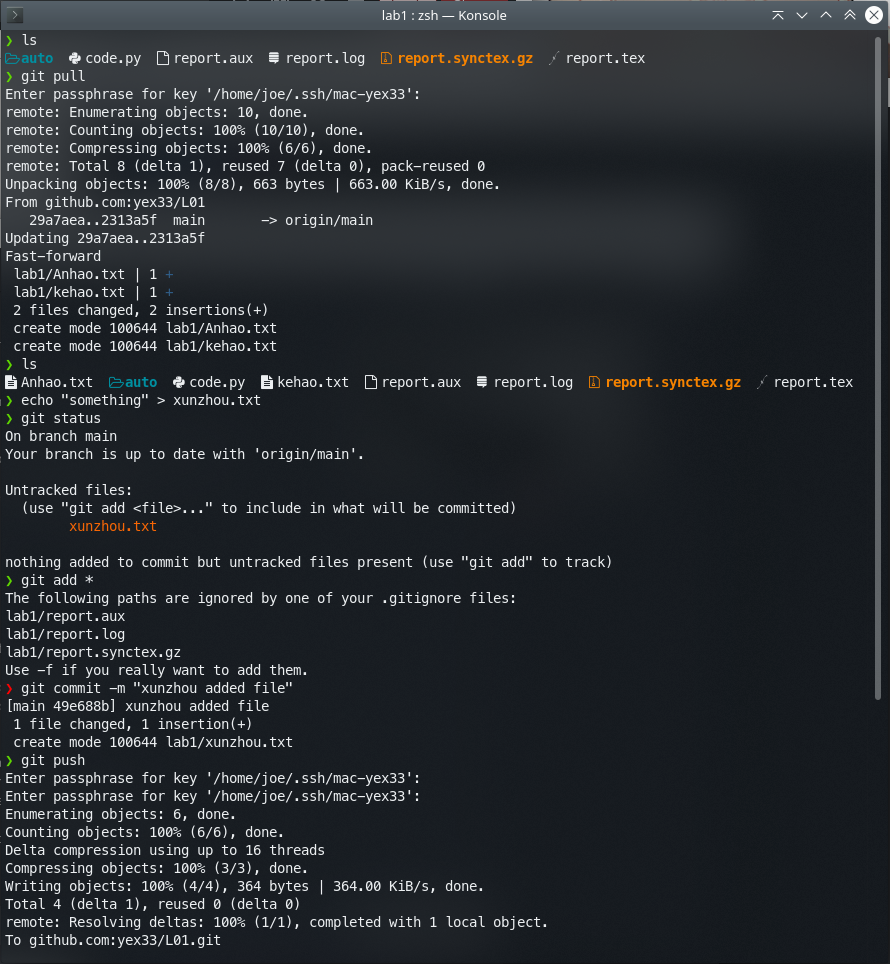
\includegraphics[width=\textwidth]{e1m3}
  \caption{Member 3}
\end{figure}

\newpage{}

\subsection{Experiment 2: Revert and Reset}

The git revert command can be considered an 'undo' type command, however, it is
not a traditional undo operation. Instead of removing the commit from the
project history, it figures out how to invert the changes introduced by the
commit and appends a new commit with the resulting inverse content. This
prevents Git from losing history, which is important for the integrity of your
revision history and for reliable collaboration.

Reverting should be used when you want to apply the inverse of a commit from
your project history. This can be useful, for example, if you’re tracking down a
bug and find that it was introduced by a single commit. Instead of manually
going in, fixing it, and committing a new snapshot, you can use git revert to
automatically do all of this for you.

The git reset command is a complex and versatile tool for undoing changes. It
has three primary forms of invocation. These forms correspond to command line
arguments --soft, --mixed, --hard. The three arguments each correspond to Git's
three internal state management mechanism's, The Commit Tree (HEAD), The Staging
Index, and The Working Directory.

\end{document}
